\section{錐の定義}
特徴ベクトル空間でサンプルベクトルが張る凸錐は以下で定義される.
\begin{equation}
	C:=\left\{\bm x|\bm x=\sum_{i=1}^{N}c_i\bm \xi_i=\Xi\bm c, \bm c\geq \bm 0\right\}
\end{equation}
ここで$N$は錐の基底ベクトル$\bm \xi_i\in\mathbb{R}^d$の数,$c_i$は非負の結合係数,$\Xi=[\bm \xi_1~\bm \xi_2~...~\bm \xi_N]$,$\bm c={}^t(c_1, c_2,.., c_N)$である.
錐は部分空間における結合係数に非負制約を課したものであり,部分空間と同様にスケール変化・ベクトルの加法に対して閉じた表現となっている.

\section{錐への角度}
錐制約部分空間法では,入力ベクトルと各クラスの錐とのなす角度によって分類を行う.角度$\theta$は入力特徴ベクトル$\bm y$とその錐$C$への正射影ベクトルのなす角度で定義される.
\begin{equation}
	\theta = \arcsin\left(\min_{\bm x\in C}\frac{\|\bm y-\bm x\|}{\|\bm y\|}\right)=\arcsin\left(\frac{1}{\|\bm y\|}\sqrt{\min_{\bm c\geq \bm 0}\|\bm y-\Xi\bm c\|^2}\right)
\end{equation}
ここで$0\leq\theta\leq\frac{\pi}{2}$である.
これは非負値最小二乗法を適用することで得られる.

\section{錐の構成方法}
凸錐の構成方法については様々な手法が提案されている\cite{cone-sub}が,本研究では非負値行列因子分解(Nonnegative Matrix Factrolization:NMF)\cite{nmf}による手法と,特徴ベクトルを包括する凸錐を構成する手法を採用した.
以下に概略を示す.
\subsection{NMFによる錐の構成}
NMFは$n\times m$の非負値行列$V$を$n\times r$の非負値行列$W$と$r\times m$の非負値行列$H$の行列積で表現する手法である.
$V=(v_{ij}),W=(w_{ij}),H=(h_{ij})$とし,$V,W,H$の$j$列目の列ベクトルをそれぞれ$\bm v_j={}^t(v_{1j}, ..., v_{nj}),\bm w_j={}^t(w_{1j}, ..., w_{nj}),\bm h_j={}^t(h_{1j}, ..., h_{rj})$と表すと,$\bm v_j$については
\begin{equation}
	\bm v_j\approx W\bm h_j=h_{1j}\bm w_{1}+h_{2j}\bm w_2+\cdots+h_{rj}\bm w_{r}
\end{equation}
と表され,$V$の列ベクトル$\bm v_j$を$W$の$r$個の列ベクトルの線形結合で近似しており,その結合係数が$\bm h_j$となる.
このため,分解後の行列$W$には錐の基底ベクトルが格納される.

\subsection{包括凸錐の構成}
\begin{figure}[htb]
	\centering
	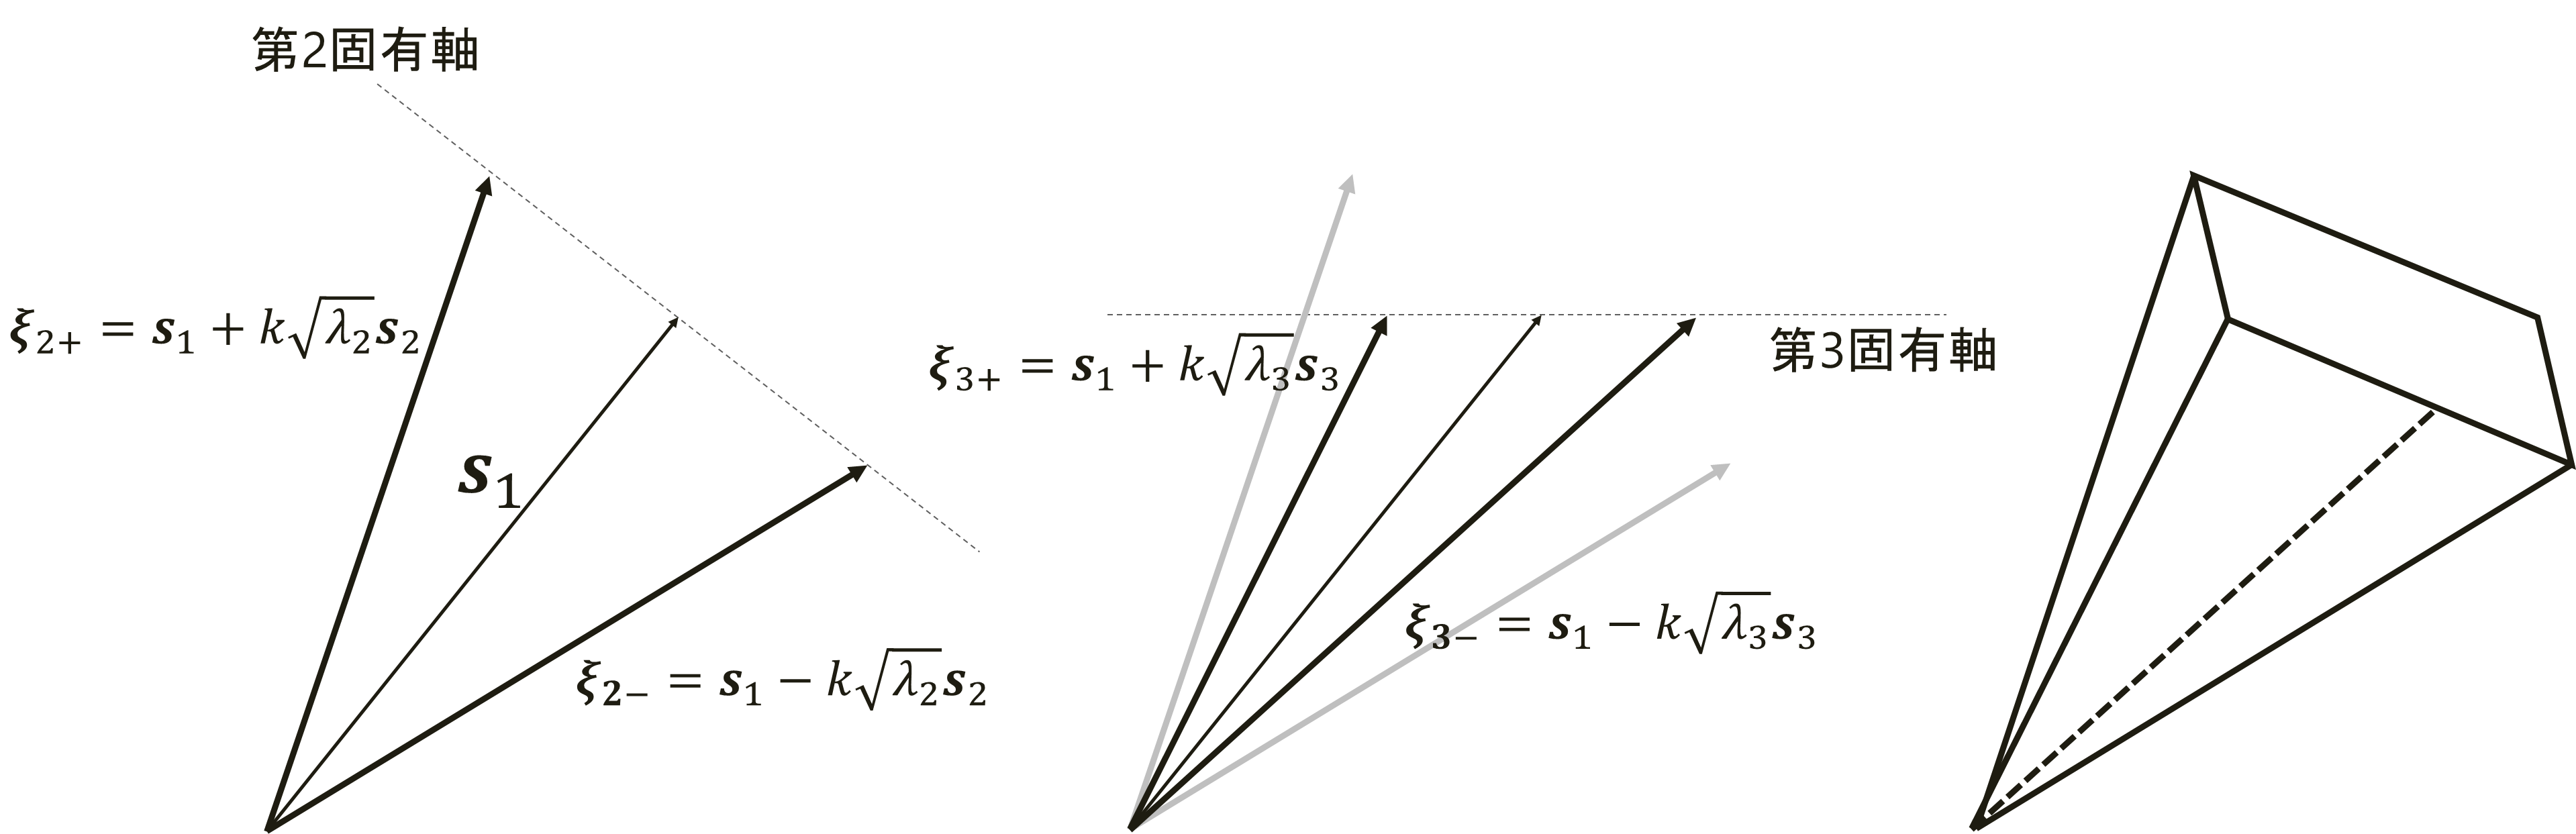
\includegraphics[width=0.7\linewidth]{image/comprehensive_cone}
	\caption{包括凸錐の構成方法(3次元空間での例)}
	\label{fig:comprehensivecone}
\end{figure}

錐のモデルとして\cite{cone-sub}は厳密な凸錐,包括凸錐,円錐を提案しているが,本研究では近似精度と計算量のバランスが良い包括凸錐を扱う.
包括凸錐は特徴ベクトル集合のなす凸錐を少数の基底ベクトルからなる包括的な凸錐で近似する手法である.
先ず,特徴ベクトル$\bm x_i\in\mathbb{R}^d$を単位超球面上に射影する.
\begin{equation}
	\bm z_i=\frac{\bm x_i}{\|\bm x_i\|}
\end{equation}
次に$\bm z_i$の自己相関行列に主成分分析(PCA)を適用する.
これにより得られた固有ベクトルを固有値の大きさに従い降順に並べたとき,第1固有ベクトルは原点からの凸錐の方向(中心),それに直交する第2以降の固有ベクトルは超球面上の特徴ベクトル集合の分布の広がりとなる.
この分布を包括する凸包は第2以降の各固有軸上で分布を包括する(分布の端点などの)2点$(\bm x_L,\bm x_R)$を選ぶことによって構成される.
つまり,各固有軸$(i\geq 2)$に対して次の2つの錐の基底ベクトルが定まる.
\begin{equation}
	\bm \xi_{i-}=\bm s_1+x_L^i\bm s_i=\bm s_1-k\sqrt{\lambda_i}\bm s_i
\end{equation}
\begin{equation}
\bm \xi_{i+}=\bm s_1+x_R^i\bm s_i=\bm s_1+k\sqrt{\lambda_i}\bm s_i
\end{equation}
ここで,$\bm s_i, \lambda_i$はそれぞれ第$i$固有ベクトル,固有値となり,$k$はスケーリングのパラメータである.
第1固有ベクトルが錐の中心ベクトルとなることから,第2以降の固有軸上での分布は原点が中心となり,その分散は固有値$\lambda_i$で与えられる.
ここでは外れ値の影響を考慮し,各軸上で標準偏差の$k$倍の点を選んでいる.